% Source: StudentGovernmentRepo/Common_Sense_Carolina_Lobbying_org/figures/information_flow.tex
\documentclass[border=5pt]{standalone}
\usepackage{tikz}
\usepackage{xcolor}
\usetikzlibrary{positioning, arrows.meta}
\definecolor{garnet}{HTML}{73000A}
\definecolor{sandstorm}{HTML}{FFF2E3}
\definecolor{rose}{HTML}{CC2E40}
\definecolor{atlantic}{HTML}{466A9F}
\definecolor{congaree}{HTML}{1F414D}
\definecolor{horseshoe}{HTML}{65780B}
\definecolor{honeycomb}{HTML}{A49137}
\definecolor{warmgrey}{HTML}{676156}

\begin{document}
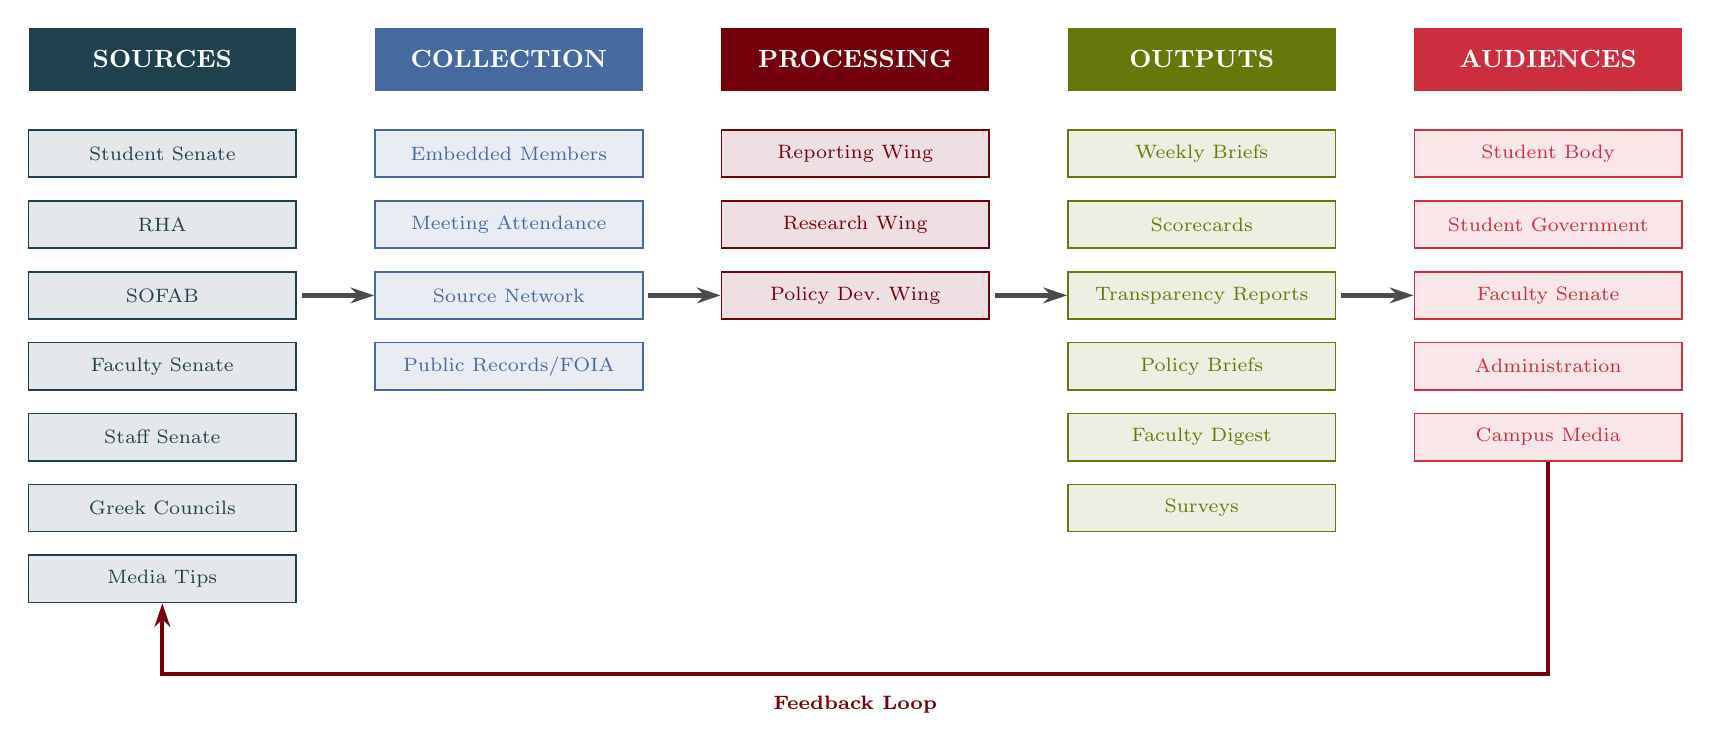
\begin{tikzpicture}[
  every node/.style={sharp corners},
  hdr/.style n args={1}{
    rectangle, fill=#1, text=white,
    font=\small\bfseries, minimum width=3.4cm, minimum height=0.8cm,
    align=center, inner sep=2pt
  },
  cell/.style n args={1}{
    rectangle, fill=#1!12, draw=#1, line width=0.6pt,
    font=\scriptsize, text=#1,
    minimum width=3.4cm, minimum height=0.6cm,
    align=center, inner sep=2pt
  },
  flowarrow/.style={
    line width=1.6pt, -{Stealth[length=3mm, width=2mm]}, color=black!70
  },
  feedarrow/.style={
    line width=1.4pt, -{Stealth[length=3mm, width=2mm]}, color=garnet
  }
]

%% Column x-positions (4.4cm apart)
\def\xA{0}
\def\xB{4.4}
\def\xC{8.8}
\def\xD{13.2}
\def\xE{17.6}

\def\rowsp{0.9}
\def\topoff{-1.2}

%% === COLUMN HEADERS (y=0) ===
\node[hdr={congaree}]  at (\xA, 0) {SOURCES};
\node[hdr={atlantic}]  at (\xB, 0) {COLLECTION};
\node[hdr={garnet}]    at (\xC, 0) {PROCESSING};
\node[hdr={horseshoe}] at (\xD, 0) {OUTPUTS};
\node[hdr={rose}]      at (\xE, 0) {AUDIENCES};

%% === COLUMN 1: SOURCES (7 items) ===
\node[cell={congaree}] (s1) at (\xA, \topoff - 0*\rowsp) {Student Senate};
\node[cell={congaree}] (s2) at (\xA, \topoff - 1*\rowsp) {RHA};
\node[cell={congaree}] (s3) at (\xA, \topoff - 2*\rowsp) {SOFAB};
\node[cell={congaree}] (s4) at (\xA, \topoff - 3*\rowsp) {Faculty Senate};
\node[cell={congaree}] (s5) at (\xA, \topoff - 4*\rowsp) {Staff Senate};
\node[cell={congaree}] (s6) at (\xA, \topoff - 5*\rowsp) {Greek Councils};
\node[cell={congaree}] (s7) at (\xA, \topoff - 6*\rowsp) {Media Tips};

%% === COLUMN 2: COLLECTION (4 items) ===
\node[cell={atlantic}] (c1) at (\xB, \topoff - 0*\rowsp) {Embedded Members};
\node[cell={atlantic}] (c2) at (\xB, \topoff - 1*\rowsp) {Meeting Attendance};
\node[cell={atlantic}] (c3) at (\xB, \topoff - 2*\rowsp) {Source Network};
\node[cell={atlantic}] (c4) at (\xB, \topoff - 3*\rowsp) {Public Records/FOIA};

%% === COLUMN 3: PROCESSING (3 items) ===
\node[cell={garnet}] (p1) at (\xC, \topoff - 0*\rowsp) {Reporting Wing};
\node[cell={garnet}] (p2) at (\xC, \topoff - 1*\rowsp) {Research Wing};
\node[cell={garnet}] (p3) at (\xC, \topoff - 2*\rowsp) {Policy Dev.\ Wing};

%% === COLUMN 4: OUTPUTS (6 items) ===
\node[cell={horseshoe}] (o1) at (\xD, \topoff - 0*\rowsp) {Weekly Briefs};
\node[cell={horseshoe}] (o2) at (\xD, \topoff - 1*\rowsp) {Scorecards};
\node[cell={horseshoe}] (o3) at (\xD, \topoff - 2*\rowsp) {Transparency Reports};
\node[cell={horseshoe}] (o4) at (\xD, \topoff - 3*\rowsp) {Policy Briefs};
\node[cell={horseshoe}] (o5) at (\xD, \topoff - 4*\rowsp) {Faculty Digest};
\node[cell={horseshoe}] (o6) at (\xD, \topoff - 5*\rowsp) {Surveys};

%% === COLUMN 5: AUDIENCES (5 items) ===
\node[cell={rose}] (a1) at (\xE, \topoff - 0*\rowsp) {Student Body};
\node[cell={rose}] (a2) at (\xE, \topoff - 1*\rowsp) {Student Government};
\node[cell={rose}] (a3) at (\xE, \topoff - 2*\rowsp) {Faculty Senate};
\node[cell={rose}] (a4) at (\xE, \topoff - 3*\rowsp) {Administration};
\node[cell={rose}] (a5) at (\xE, \topoff - 4*\rowsp) {Campus Media};

%% === FORWARD ARROWS (all aligned at row 3) ===
\draw[flowarrow] (s3.east) ++(0.06,0) -- (c3.west);
\draw[flowarrow] (c3.east) ++(0.06,0) -- (p3.west);
\draw[flowarrow] (p3.east) ++(0.06,0) -- (o3.west);
\draw[flowarrow] (o3.east) ++(0.06,0) -- (a3.west);


%% === FEEDBACK LOOP (below everything) ===
%% Route: Audiences bottom-right -> down -> left across full width -> up -> Sources bottom-left
\draw[feedarrow]
  (a5.south) -- ++(0, -2.7)
  -- ++(-\xE + \xA, 0)
  -- (s7.south);

\node[font=\scriptsize\bfseries, text=garnet,
      fill=white, inner sep=2pt]
  at (8.8, -8.2) {Feedback Loop};

\end{tikzpicture}
\end{document}
